% Fig 4: Cost-benefit tradeoff scatter
\begin{figure}[t]
\centering
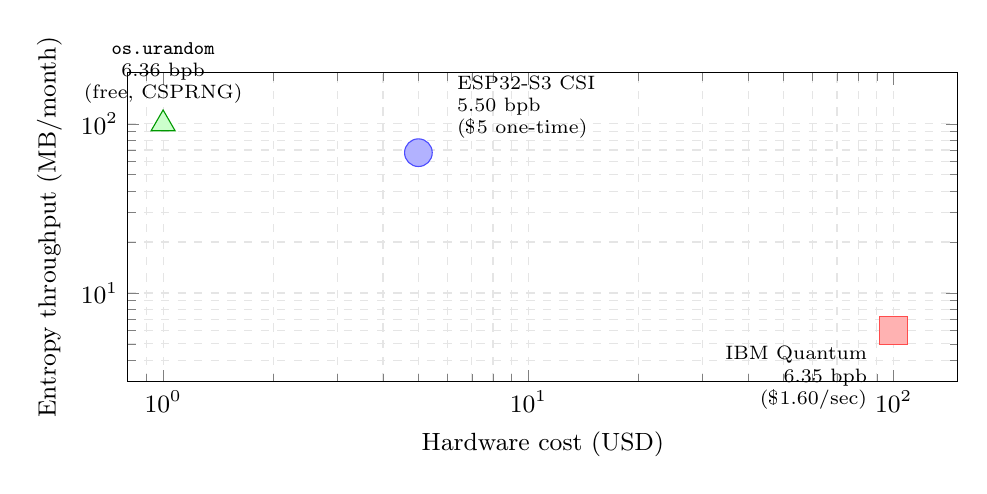
\begin{tikzpicture}
\begin{axis}[
  width=\columnwidth,
  height=5.5cm,
  xlabel={Hardware cost (USD)},
  ylabel={Entropy throughput (MB/month)},
  xlabel style={font=\small},
  ylabel style={font=\small},
  xticklabel style={font=\small},
  yticklabel style={font=\small},
  xmode=log,
  ymode=log,
  xmin=0.8, xmax=150,
  ymin=3, ymax=200,
  grid=both,
  grid style={dashed, gray!20},
  clip=false,
]

% os.urandom: $0 effective -> show at $1 with annotation
\addplot[only marks, mark=triangle*, mark size=5pt, green!60!black, fill=green!20]
  coordinates {(1, 100)};
\node[font=\scriptsize, anchor=south, align=center] at (axis cs:1, 115)
  {\texttt{os.urandom}\\6.36~bpb\\(free, CSPRNG)};

% ESP32-S3 CSI
\addplot[only marks, mark=*, mark size=5pt, blue!70, fill=blue!30]
  coordinates {(5, 67.5)};
\node[font=\scriptsize, anchor=south west, align=left] at (axis cs:6, 72)
  {ESP32-S3 CSI\\5.50~bpb\\(\$5 one-time)};

% IBM Quantum: effective amortized cost ~$100/mo for 6MB
\addplot[only marks, mark=square*, mark size=5pt, red!70, fill=red!30]
  coordinates {(100, 6)};
\node[font=\scriptsize, anchor=north east, align=right] at (axis cs:90, 5.5)
  {IBM Quantum\\6.35~bpb\\(\$1.60/sec)};

\end{axis}
\end{tikzpicture}
\caption{Cost--throughput tradeoff. CSI entropy from a \$5 ESP32-S3 produces 45--90~MB/month of genuine physical randomness at zero marginal cost, occupying a unique niche between free-but-deterministic OS entropy and high-quality-but-expensive quantum entropy. Bubble annotations show NIST SP~800-90B min-entropy.}
\label{fig:cost-benefit}
\end{figure}
